%% Template originaly created by Karol Kozioł (mail@karol-koziol.net) and modified for ShareLaTeX use

\documentclass[a4paper,11pt]{article}

\usepackage[T1]{fontenc}
\usepackage[utf8]{inputenc}
\usepackage{graphicx}
\usepackage{xcolor}
\renewcommand\familydefault{\rmdefault}
\usepackage{tgheros}

\usepackage{amsmath,amssymb,amsthm,textcomp}
\usepackage{enumerate}
\usepackage{multicol}
\usepackage{tikz}
\usepackage[utf8]{vietnam}
\usepackage[unicode]{hyperref}

\usepackage{geometry}
\geometry{total={210mm,297mm},
left=25mm,right=25mm,%
bindingoffset=0mm, top=22mm,bottom=25mm}

\linespread{1.3}

\newcommand{\linia}{\rule{\linewidth}{0.5pt}}

% custom theorems if needed
\newtheoremstyle{mytheor}
    {1ex}{1ex}{\normalfont}{0pt}{\scshape}{.}{1ex}
    {{\thmname{#1 }}{\thmnumber{#2}}{\thmnote{ (#3)}}}

\theoremstyle{mytheor}
\newtheorem{defi}{Definition}

% my own titles
\makeatletter
\renewcommand{\maketitle}{
\begin{center}
\vspace{2ex}
{\huge \textsc{\@title}}
\vspace{1ex}
\\
\linia\\
\@author \hfill \@date
\vspace{4ex}
\end{center}
}
\makeatother
%%%

% custom footers and headers
\usepackage{fancyhdr}
\setlength{\headheight}{20pt}
\pagestyle{fancy}
\fancyhead{} % clear all header fields
\fancyhead[L]{
 \begin{tabular}{rl}
    \begin{picture}(15,10)(0,0)
    \put(0,-8){
\includegraphics[width=8mm, height=8mm]{vgu_logo.png}}
    %\put(0,-8){\epsfig{width=10mm,figure=hcmut.eps}}
   \end{picture}&
	%\includegraphics[width=8mm, height=8mm]{hcmut.png} & %
	\begin{tabular}{l}
		\textbf{\bf \ttfamily Vietnamese-German University}\\
		\textbf{\bf \ttfamily Department of Computer Science}
	\end{tabular} 	
 \end{tabular}
}
\fancyhead[R]{
	\begin{tabular}{l}
		\tiny \bf \\
		\tiny \bf 
	\end{tabular}  }
\fancyfoot{} % clear all footer fields
\fancyfoot[L]{\scriptsize \ttfamily Introduction to Information Technology Project}
\rfoot{Page \thepage}
\renewcommand{\headrulewidth}{0.2pt}
\renewcommand{\footrulewidth}{0.2pt}
%



% code listing settings
\usepackage{listings}
\lstset{
    language=Python,
    basicstyle=\ttfamily\small,
    aboveskip={1.0\baselineskip},
    belowskip={1.0\baselineskip},
    columns=fixed,
    extendedchars=true,
    breaklines=true,
    tabsize=4,
    prebreak=\raisebox{0ex}[0ex][0ex]{\ensuremath{\hookleftarrow}},
    frame=lines,
    showtabs=false,
    showspaces=false,
    showstringspaces=false,
    keywordstyle=\color[rgb]{0.627,0.126,0.941},
    commentstyle=\color[rgb]{0.133,0.545,0.133},
    stringstyle=\color[rgb]{01,0,0},
    numbers=left,
    numberstyle=\small,
    stepnumber=1,
    numbersep=10pt,
    captionpos=t,
    escapeinside={\%*}{*)}
}

%%%----------%%%----------%%%----------%%%----------%%%

\begin{document}

\begin{titlepage}
\begin{center}
VIETNAMESE - GERMAN UNIVERSITY \\
DEPARTMENT OF COMPUTER SCIENCE
\end{center}

\vspace{1cm}

\begin{figure}[h!]
\begin{center}

\includegraphics[width=3cm]{vgu_logo.png}
\end{center}
\end{figure}

\vspace{2cm}


\begin{center}
\begin{tabular}{c}
%\multicolumn{1}{c}{\textbf{{\Large BÁO CÁO BÀI TẬP LỚN}}}
\multicolumn{1}{c}{\textbf{{\Large Introduction to Information Technology Project}}}



~~\\

\\
\multicolumn{1}{l}{\textbf{{\Large}}}\\
\\
\textbf{{\Large}}\\

\\
\\

\end{tabular}
\end{center}

\vspace{2cm}

\begin{table}[h]
\begin{tabular}{rrl}
&\textbf{Group:} & Lightning McQueen\\
\hspace{5.1cm} 
&\textit{Student 1: } & 10423128 - Lê Đức Anh\\
&\textit{Student 2: } & 10423130 - Trịnh Thị Như Bình\\
&\textit{Student 3: } & 10423136 - Nguyễn Bảo Thành Đạt\\
&\textit{Student 4: } & 10423163 - Hà Thiên Phúc\\
&\textit{Student 5: } & 10423172 - Nguyễn Huỳnh Kim Thoa\\
&\textit{Student 6: } & 10423173 - Trần Anh Thư\\


\end{tabular}
\end{table}
\vspace{3cm}
\begin{center}
{\footnotesize BÌNH DƯƠNG, 05/ 2023}
\end{center}
\end{titlepage}

%\thispagestyle{empty}
\renewcommand{\contentsname}{Content}
\newpage
\vspace{1cm}
\tableofcontents
\newpage

\section{Introduction}
    

In the first part of the report, students should provide briefly the idea of their project, which is based on Google Teachable Machine.




\section{Dataset Collection}

Present your dataset for each class by capturing the screen when pictures are uploaded to Google Teachable Machine tool. Please notice that number of classes is at least, equal to the number of students in your group. Moreover, the \textbf{background} class must be included in your AI.\\

\subsection{Class 1: Bike}
Bike: A bike is a two-wheeled vehicle powered by pedals. It is commonly used for transportation, exercise, or leisure. 
\begin{figure}
    \centering
    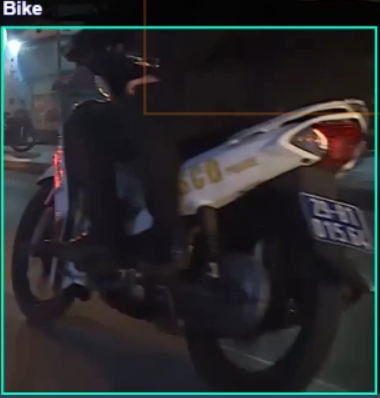
\includegraphics[width=0.5\linewidth]{bike2.png}
    \caption{Bike example}
    \label{fig:enter-label}
\end{figure}
\begin{figure}
    \centering
    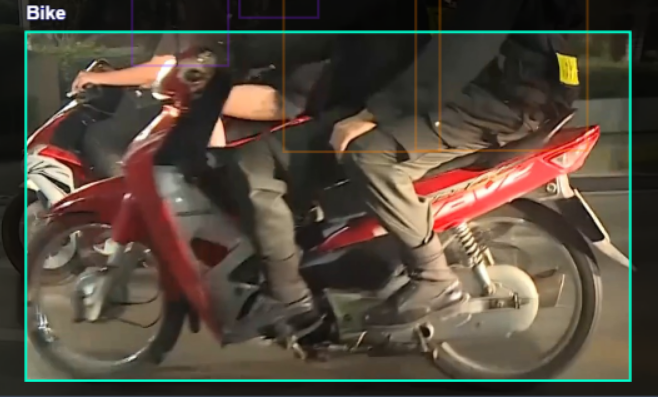
\includegraphics[width=0.5\linewidth]{images/Bike1.png}
    \caption{Bike example}
    \label{fig:enter-label}
\end{figure}
 
\subsection{Class 2: Car}
Car: A car is a four-wheeled motor vehicle designed for personal transportation. It offers convenience, speed, and comfort. 
\begin{figure}
    \centering
    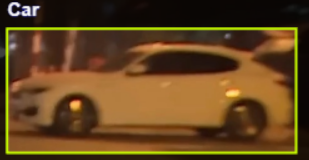
\includegraphics[width=0.5\linewidth]{images/car2.png}
    \caption{Car example}
    \label{fig:enter-label}
\end{figure}

 \begin{figure}
     \centering
     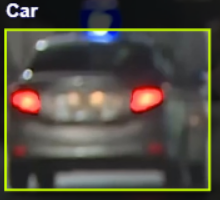
\includegraphics[width=0.5\linewidth]{images/car1.png}
     \caption{Car example}
     \label{fig:enter-label}
 \end{figure}
\subsection{Class 3: Bus}
Bus: A bus is a large motor vehicle designed to carry passengers. It is used for public transportation or group travel. 
 
\subsection{Class 4: People}
People: People refer to human  beings who  participate in road traffic.

 
\subsection{Class 5: Police}
Police: The police are law enforcement officers responsible for maintaining order and safety. They wear uniforms and carry weapons. 

\subsection{Class 6: Traffic sign}
Traffic Sign: A traffic sign is a road sign with specific shapes, colors, and symbols. These signs convey important information to drivers and pedestrians.  

\subsection{Multi-Classes:}
This part is the images for background

\section{Python Source Code}

The python source code of your project is presented in this part, for instance:

\begin{lstlisting}[language=Python, caption= Example of your Python code, label=test_float]
from keras.models import load_model  # TensorFlow is required for Keras to work
import cv2  # Install opencv-python
import numpy as np

# Disable scientific notation for clarity
np.set_printoptions(suppress=True)

# Load the model
model = load_model("keras_Model.h5", compile=False)

# Load the labels
class_names = open("labels.txt", "r").readlines()

# CAMERA can be 0 or 1 based on default camera of your computer
camera = cv2.VideoCapture(0)

while True:
    # Grab the webcamera's image.
    ret, image = camera.read()

    # Resize the raw image into (224-height,224-width) pixels
    image = cv2.resize(image, (224, 224), interpolation=cv2.INTER_AREA)

    # Show the image in a window
    cv2.imshow("Webcam Image", image)

    # Make the image a numpy array and reshape it to the models input shape.
    image = np.asarray(image, dtype=np.float32).reshape(1, 224, 224, 3)

    # Normalize the image array
    image = (image / 127.5) - 1

    # Predicts the model
    prediction = model.predict(image)
    index = np.argmax(prediction)
    class_name = class_names[index]
    confidence_score = prediction[0][index]

    # Print prediction and confidence score
    print("Class:", class_name[2:], end="")
    print("Confidence Score:", str(np.round(confidence_score * 100))[:-2], "%")

    # Listen to the keyboard for presses.
    keyboard_input = cv2.waitKey(1)

    # 27 is the ASCII for the esc key on your keyboard.
    if keyboard_input == 27:
        break

camera.release()
cv2.destroyAllWindows()

\end{lstlisting}

\section{Implementing}

\subsection{Model Evaluation:}
\subsection{Result:}

\section{Extra Features:}
Your extra features can be listed in this part

\subsection{Extra function 1:}
Another extra function if it is available. 

\subsection{Extra function 2:}
Another extra function if it is available. 

\section{Conclusion}
Put some conclusions in this part

%%%%%%%%%%%%%%%%%%%%%%%%%%%%%%%%%
% \newpage
% \addcontentsline{toc}{section}{Reference}
% \begin{thebibliography}{99999}

% \bibitem[Web]{1}{Arduino,} {\url{https://www.arduino.cc/}}


% \end{thebibliography}
\end{document}
